\documentclass[a4paper, 12pt]{article}
\usepackage[a4paper, margin=2.5cm]{geometry} % Margins
\usepackage{amsmath, amssymb}
\usepackage{graphicx}
\usepackage{hyperref}
\usepackage{float}
\usepackage{color}
\usepackage{subcaption}
\usepackage{fancyhdr}
\usepackage{tcolorbox} % For boxed environment
\usepackage{setspace}

% Header and footer setup
\pagestyle{fancy}
\fancyhf{}
\fancyhead[L]{\textbf{Deep Learning – Homework 2}}
\fancyhead[R]{Group 14}
\fancyfoot[C]{\thepage}

% Title and author customization
\title{\textbf{Deep Learning (IST, 2024-25) \\ Homework 2}}
\author{Luís Calado - 103883 \& Salvador Florêncio - 102706}
\date{}

\begin{document}

\maketitle
\vspace{-0.8cm}
\begin{center}
    \textbf{Group 14}
\end{center}

%\vspace{0.1 cm}

% Contribution box
\begin{tcolorbox}[colframe=black, colback=white, sharp corners, boxrule=1pt, width=\textwidth]

\textbf{IMPORTANT:} Both members of the group were involved in the resolution of all questions in the homework.
\end{tcolorbox}

%\vspace{1cm}

\maketitle

\section*{Question 1}

\subsection*{1.}
One may start by defining $E_1$ and $E_2$ as suggested: $E_1(\mathbf{q}) = \frac{1}{2} \mathbf{q}^\top \mathbf{q} + \beta^{-1} \log N + \frac{1}{2} M^2 \hspace{0.2cm}
\text{and} \hspace{0.2cm}
E_2(\mathbf{q}) = -\mathrm{lse}(\beta, \mathbf{X}\mathbf{q})$. For $\nabla E_1(\mathbf{q})$ one may see that:
\[
\nabla E_1(\mathbf{q}) = \nabla_{\mathbf{q}} \left( \frac{1}{2} \mathbf{q}^\top \mathbf{q} + C \right) = \nabla_{\mathbf{q}} \left( \frac{1}{2} \mathbf{q}^\top \mathbf{q} \right) = \frac{1}{2} \nabla_{\mathbf{q}} \left( \mathbf{q}^\top \mathbf{q} \right) 
= \frac{1}{2} \cdot 2 \mathbf{q} = \mathbf{q}. 
\]
As for $\nabla(- E_2(\mathbf{q}))$, one can see: 
\[
\nabla(- E_2(\mathbf{q})) = \nabla_{\mathbf{q}} \left( \text{lse}(\beta \mathbf{X}\mathbf{q})\right) 
= \nabla_{\mathbf{q}} \left( \beta^{-1} \log \sum_{i=1}^N \exp(\beta X_iq) \right) 
\]

\[
=\beta^{-1}\nabla_{\mathbf{q}} \left( \log \sum_{i=1}^N \exp(\beta X_iq) \right) 
\]

\[
= \beta^{-1}\frac{\nabla_{\mathbf{q}} \left( \sum_{i=1}^N \exp(\beta X_iq) \right)}{\sum_{i=1}^N \exp(\beta X_iq)} = \frac{ \left(  X_1\exp(\beta X_1q) + ... + X_N\exp(\beta X_Nq) \right)}{\sum_{i=1}^N \exp(\beta X_iq)}
\]

\[
= \frac{\sum_{i=1}^N X_i \exp(\beta X_iq)}{\sum_{i=1}^N \exp(\beta X_iq)} = X^\top \text{softmax}(\beta Xq)
\]
To compute the Hessians of $E_1$ and $-E_2$, one have: \[
   \nabla^2( E_1(\mathbf{q}) )= I \quad (\text{positive definite}),
   \]
    \[
   \nabla^2(-E_2(\mathbf{q})) = \beta X^\top \left( \text{diag}(p) - pp^\top \right) X, \hspace{0.2cm}\beta>0 \quad p=\text{softmax}(\beta Xq)\quad \footnote{The jacobian of the softmax function was omited, but is referenced in the paper cited in \cite{unknown}.}(\text{positive semi-definite}).
   \]
   In the case of $\nabla^2( E_1(\mathbf{q}) )$, it's immediately positive definite because it is diagonal with all diagonal entries equal to 1 (symmetric diagonally dominant matrix with non-negative diagonal elements). For $\nabla^2( -E_2(\mathbf{q}) )$, one may use Jensen’s inequality to prove that $\nabla^2( E_2(\mathbf{q}) )$ is psd: 
   \[X^T (\text{diag}(p) - pp^T) X = \sum_i p_i x_i^2 - \left( \sum_i p_i x_i \right)^2 =  \sum_i p_i g(x_i) - g\left( \sum_i p_i x_i \right) \geq 0, 
    \]
    With $g(x)=x^2$ being a convex function, \( g : \mathbb{R} \to \mathbb{R} \). Thus, lse is convex and $-$lse (i.e, $E_2(\mathbf{q})$) is a concave function.

   Therefore, the energy function $E(\mathbf{q})$ is the sum of the convex function $E_1(\mathbf{q})$ and the concave function $E_2(\mathbf{q})$ \cite{unknown}.
\subsection*{2.}
The concave function \( E_2(\mathbf{q}) \) is approximated using a first-order Taylor expansion around \( \mathbf{q}_t \):
\[
E_2(\mathbf{q}) \approx \tilde{E}_2(\mathbf{q}) := E_2(\mathbf{q}_t) + (\nabla E_2(\mathbf{q_t}))^\top (\mathbf{q} - \mathbf{q}_t).
\]From earlier calculations, the gradient of \( E_2(\mathbf{q}) \) is:
\[
\nabla E_2(\mathbf{q}) = -X^\top \text{softmax}(\beta X \mathbf{q}).
\]
Substituting this gradient:
\[
\tilde{E}_2(\mathbf{q}) := E_2(\mathbf{q}_t) - \left( X^\top \text{softmax}(\beta X \mathbf{q}_t) \right)^\top (\mathbf{q} - \mathbf{q}_t).
\]
The next iterate \( \mathbf{q}_{t+1} \) is computed by solving the following convex optimization problem:
\[
\mathbf{q}_{t+1} = \arg \min_{\mathbf{q}} E_1(\mathbf{q}) + \tilde{E}_2(\mathbf{q}).
\]
Substituting \( E_1(\mathbf{q}) \) and \( \tilde{E}_2(\mathbf{q}) \), we have:
\[
E_1(\mathbf{q}) + \tilde{E}_2(\mathbf{q}) = \frac{1}{2} \mathbf{q}^T\mathbf{q} + C - \left( X^\top \text{softmax}(\beta X \mathbf{q}_t) \right)^\top \mathbf{q},
\]
where \( C \) is a constant that does not depend on \( \mathbf{q} \) (and thus can be ignored for the optimization). The optimization problem becomes:
\[
\mathbf{q}_{t+1} = \arg \min_{\mathbf{q}} \frac{1}{2} \mathbf{q}^T\mathbf{q} - \left( X^\top \text{softmax}(\beta X \mathbf{q}_t) \right)^\top \mathbf{q}.
\]
To solve this, compute the gradient of the objective function with respect to \( \mathbf{q} \) and set it to zero:
\[
\nabla_\mathbf{q} \left( \frac{1}{2} \mathbf{q}^T\mathbf{q}- \left( X^\top \text{softmax}(\beta X \mathbf{q}_t) \right)^\top \mathbf{q} \right) = 0.
\]
The gradient is:
\[
\nabla_\mathbf{q} \left( \frac{1}{2} \mathbf{q}^T\mathbf{q} \right) = \mathbf{q},
\]
\[
\nabla_\mathbf{q} \left( -\left( X^\top \text{softmax}(\beta X \mathbf{q}_t) \right)^\top \mathbf{q} \right) = -X^\top \text{softmax}(\beta X \mathbf{q}_t).
\]
Setting the gradient to zero:
\[
\mathbf{q} - X^\top \text{softmax}(\beta X \mathbf{q}_t) = 0.
\]
Thus, applying the CCCP algorithm to the Hopfield energy function yields the update rule:
\[
\mathbf{q}_{t+1} = X^\top \text{softmax}(\beta X \mathbf{q}_t).
\]
\subsection*{3.}
For $N$ memory patterns $\mathbf{Q} = \begin{bmatrix} \mathbf{q}_t^{(1)},  \cdots, \mathbf{q}_t^{(N)} \end{bmatrix}^T$, the update rule can be generalized to:
\[
(Q^{new})^T = X^T \text{softmax}(\beta X Q^T)
\]
We first consider $X$ as $N$ raw stored patterns $Y = [y_1,..., y_N]^T$, which are mapped to an associative space via $W_K$, and $Q$ as $S$ raw state patterns $R = [y_1,..., y_N]^T$, which are mapped to an associative space via $W_Q$. Setting, 
\[
Q=RW_Q,
\]
\[
K=X=YW_K, 
\]
\[
\beta= \frac{1}{\sqrt{D}},
\]
we obtain:
\[
(Q^{new})^T = K^T \text{softmax}\left(\frac{1}{\sqrt{D}} K Q^T \right).
\]
Next, we simple transpose and obtain:
\[
Q^{new} = \text{softmax}\left(\frac{1}{\sqrt{D}} Q K^T\right)K.
\]
Now, we only need to project $Q^{new}$ via another projection matrix $W_V$:
\[
Z= Q^{new}W_V = \text{softmax}\left(\frac{1}{\sqrt{D}} Q K^T\right)KW_V = \text{softmax}\left(\frac{1}{\sqrt{D}} Q K^T\right) V,
\]
and we have obtained the transformer attention \cite{brandstetter2020hopfield}. For a single query vector $q_t$ (a row of $Q$), the cross-attention computation simplifies to:
\[
q_{t+1}= \text{softmax} \left( \frac{q_t X^T}{\sqrt{D}} \right) X.
\]
The Hopfield update is mathematically equivalent to the transformer's cross-attention computation, with a key difference in how rows and columns of $X$ are interpreted. In a Hopfield network, the focus is on the columns of $X$ (representing memory patterns), whereas in a transformer, the focus is on the rows of $X$ (representing sequence elements).
\section*{Question 2}
\subsection*{1.}
Training 40 epochs with a learning rate of 0.01 (the best configuration) and using the SGD optimizer we get a validation accuracy of 0.6937 and a final test accuracy of 0.6927.


\begin{figure}[H]
    \centering
    % First image
    \begin{subfigure}{0.45\linewidth}
        \centering
        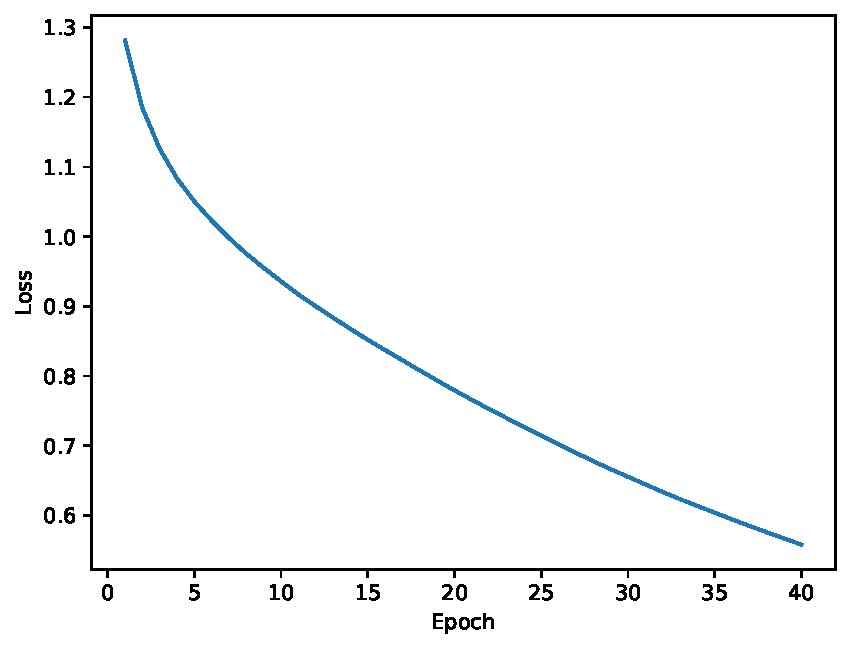
\includegraphics[width=\linewidth]{plot/q2/CNN-3-train-loss-40-8-0.01-0-0.1-sgd-False-True-69.27.pdf}
        \caption{Average train loss as a function
of the epoch number.}
        \label{fig:loss_0.01}
    \end{subfigure}
    % Spacer between images
    \hspace{0.05\linewidth}
    % Second image
    \begin{subfigure}{0.45\linewidth}
        \centering
        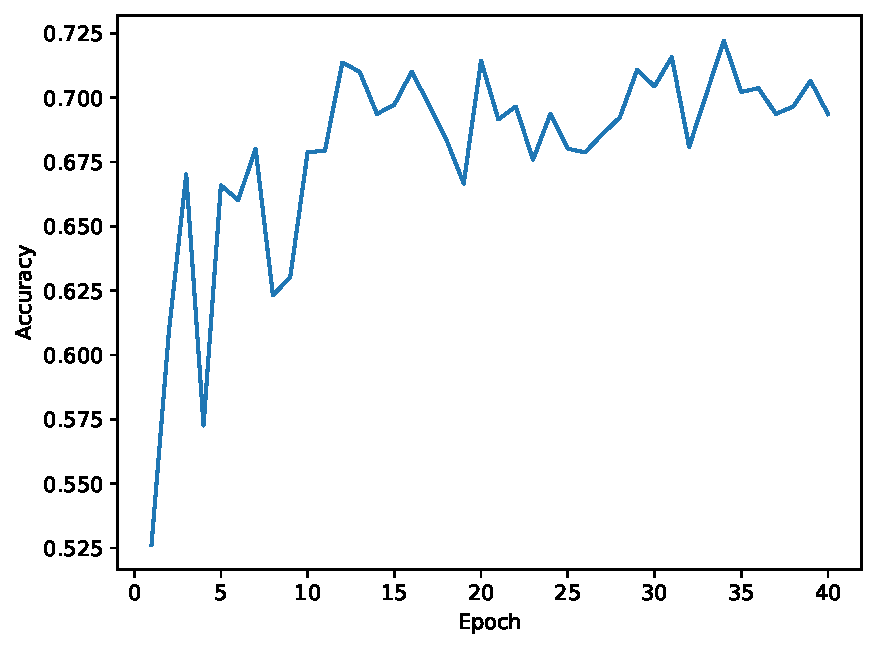
\includegraphics[width=\linewidth]{plot/q2/CNN-3-valid-accuracy-40-8-0.01-0-0.1-sgd-False-True-69.27.pdf}
        \caption{Validation accuracy as a function of the epoch number.}
        \label{fig:acc_0.01}
    \end{subfigure}
    \caption{CNN performance over 40 epochs with a learning rate of 0.01 (best configuration).}
    \label{fig:side-by-side1}
\end{figure}

\subsection*{2.}
Training 40 epochs with a learning rate of 0.01, a l2 weight decay of 0, a dropout probability of 0.1, using the SGD optimizer, batch normalization in each convolutional block, a global average pooling layer and a batch normalization layer in the MLP block we get a validation accuracy of 0.7365 and a final test accuracy of 0.7460. 
\begin{figure}[H]
    \centering
    % First image
    \begin{subfigure}{0.45\linewidth}
        \centering
        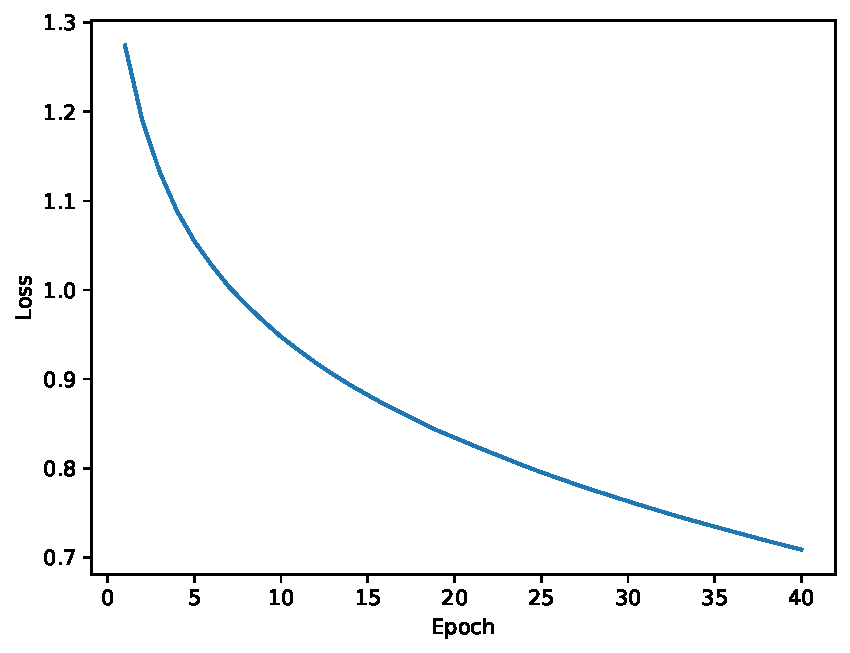
\includegraphics[width=\linewidth]{plot/q2/CNN-3-train-loss-40-8-0.01-0-0.1-sgd-False-False-74.60.pdf}
        %\caption{Average train loss as a function of the epoch number.}
        \label{fig:batch_loss_0.01}
    \end{subfigure}
    % Spacer between images
    \hspace{0.05\linewidth}
    % Second image
    \begin{subfigure}{0.45\linewidth}
        \centering
        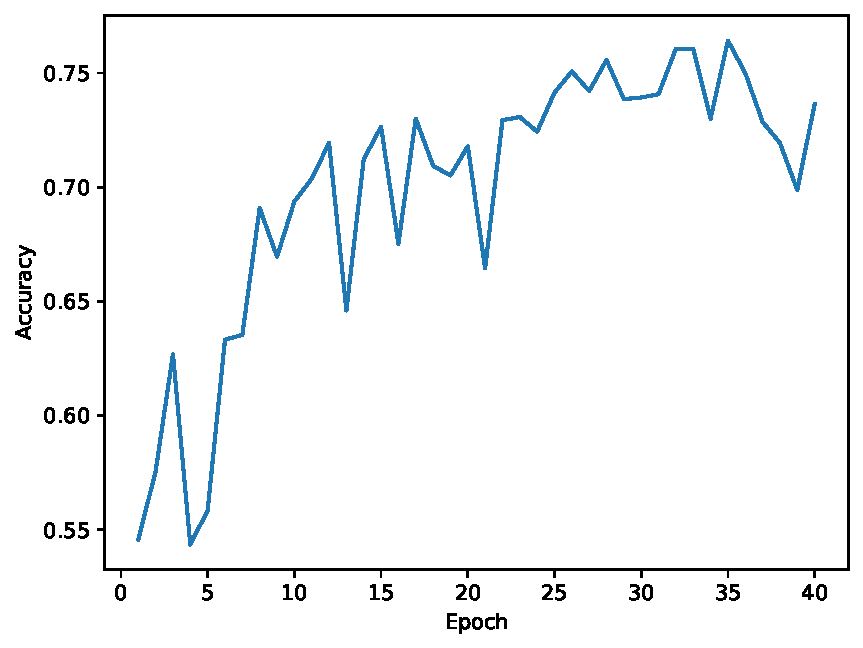
\includegraphics[width=\linewidth]{plot/q2/CNN-3-valid-accuracy-40-8-0.01-0-0.1-sgd-False-False-74.60.pdf}
        %\caption{Validation accuracy as a function of the epoch number.}
        \label{fig:batch_acc_0.01}
    \end{subfigure}
    \vspace{-0.4cm}
    \caption{CNN performance with the best model (with a learning rate of 0.01) as a function of the epoch number. On the right: average train loss. On the left: validation accuracy. }
\end{figure}
\subsection*{3.}
The number of trainable parameters is the modified version of the CNN is 755718 whereas for the previous version was 5342790. This reduction is primarily due to replacing the flattening operation with global average pooling, which reduces the input size to the MLP block (4608 vs 128). Additionally, while batch normalization introduces some parameters, their impact is minimal compared to the size of the fully connected layers.

The smaller parameter count in the modified network helps prevent overfitting and improves generalization, as evidenced by its performance. The addition of batch normalization further stabilizes training and allows for better optimization, making the modified CNN not only more efficient but also more effective despite having fewer parameters.
%With the same capacity, the justification for the difference found in terms of performance
%for the two networks is the use of the max-pooling layers that improve invariance ensuring that if there is a small translation of the input, the values of the pooled outputs remain
%unchanged.
\subsection*{4.} 

Small kernels have fewer parameters when compared to larger kernels (width x height), this reduces the computational cost and makes training more efficient. Another advantage of smaller kernels is the ability to efficiently capture local patterns.\vspace{0.3cm} \\ 
Pooling layers allow to reduce the dimensional space. Pooling layers provide invariance by summarizing features within a region of the feature map, rather than relying on their exact positions. This allows the model to focus on key features, making it more robust to variations in feature position within the input image.

\section*{Question 3}
\subsection*{1.a)}
\vspace{-0.8cm}
\begin{figure}[H]
    \centering
    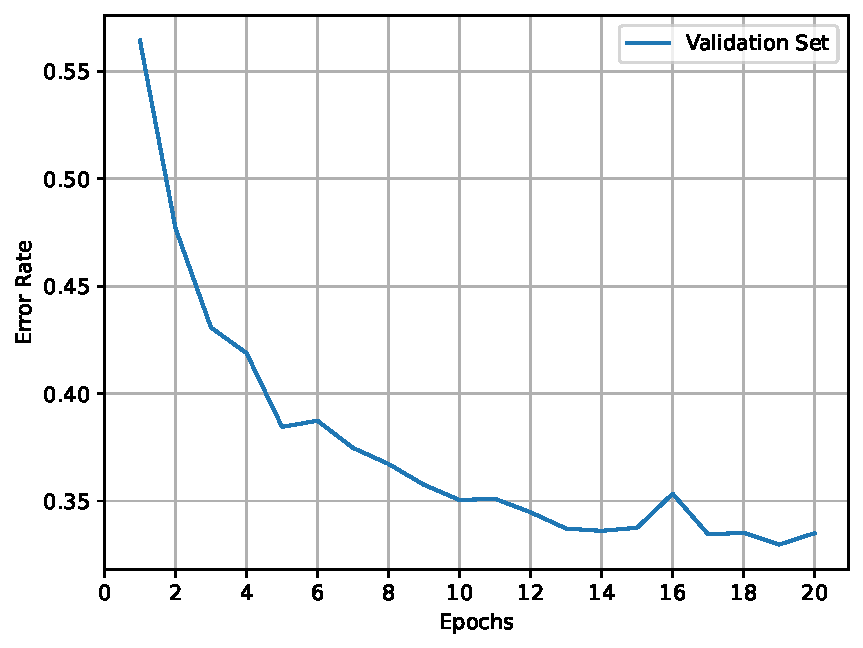
\includegraphics[width=0.8\textwidth]{plot/q3/attn_False_err_rate.pdf}
    \caption{Seq2Seq: Character Error Rate (CER) on the validation set as a function of the epoch number.}
\end{figure}

After training our model for 20 epochs using a learning rate of 0.003, a dropout rate of 0.3, a hidden size of 128, and a batch size of 64; on the test set, our model achieved a Character Error Rate (CER) of 0.3177, and a Word Error Rate (WER) of 0.8280.

\subsection*{1.b) Bahdanau Attention} 
\vspace{-0.8cm}
\begin{figure}[H]
    \centering
    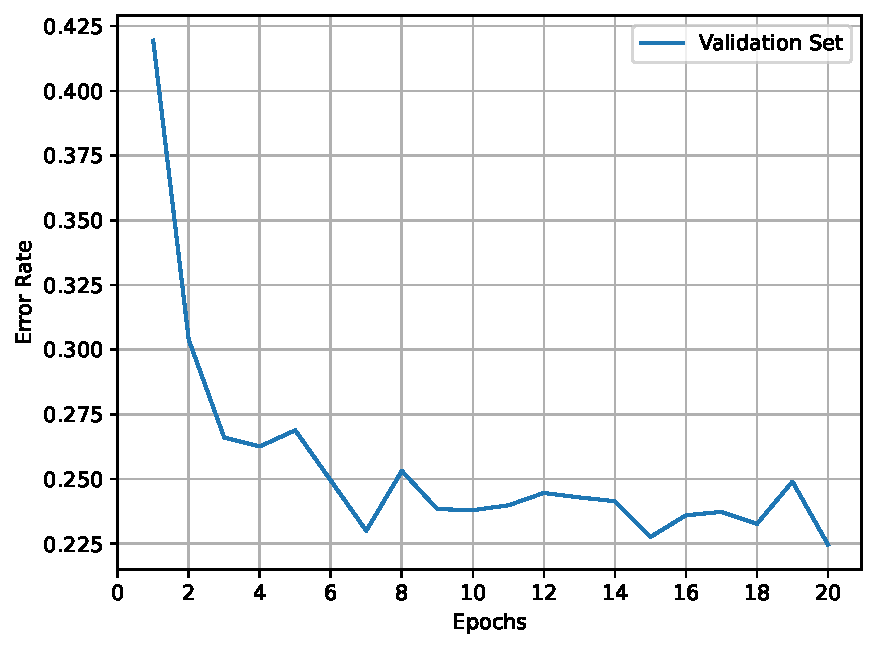
\includegraphics[width=0.8\textwidth]{plot/q3/attn_True_err_rate.pdf}
    \caption{Seq2Seq: Character Error Rate (CER) on the validation set as a function of the epoch number, with the Bahdanau Attention mechanism. }
\end{figure}
After training our model for 20 epochs using a learning rate of 0.003, a dropout rate of 0.3, a hidden size of 128, and a batch size of 64; on the test set, our model achieved a Character Error Rate (CER) of 0.2199, and a Word Error Rate (WER) of  0.7450. 


\subsection*{1.c)}

After implementing the \texttt{nucleus\_sampling} function to generate new predictions for our model with attention mechanism from part (b) and  top-p sampling, we obtained a test Character Error Rate (CER) of 0.2464, a Word Error Rate (WER) of 0.7650, and a WER@3 of 0.6640.

\bibliography{refs} 
\bibliographystyle{plain} 
\end{document}

